\documentclass[11pt]{article}

% --- Packages (all in a standard TeX Live / arXiv environment) ---
\usepackage[utf8]{inputenc}
\usepackage[T1]{fontenc}
\usepackage{lmodern}
\usepackage[margin=1in]{geometry}
\usepackage{microtype}
\usepackage{graphicx}
\usepackage{booktabs}
\usepackage{xcolor}
\usepackage{listings}
\usepackage[round]{natbib}
\usepackage{hyperref}
\hypersetup{colorlinks=true, linkcolor=black, citecolor=blue, urlcolor=blue}
\bibliographystyle{plainnat}

% --- Code listing style (R) ---
\definecolor{codegray}{gray}{0.95}
\lstset{
  basicstyle=\ttfamily\small,
  backgroundcolor=\color{codegray},
  frame=single,
  framesep=4pt,
  rulecolor=\color{gray!40},
  breaklines=true,
  columns=fullflexible,
  keepspaces=true,
  showstringspaces=false,
  language=R,
  keywordstyle=\color{black},
  commentstyle=\itshape\color{gray!70!black},
}

\title{\textbf{reaborn}: A faithful R port of seaborn\\ built on the grammar of graphics}
\author{
  Shawn T. Schwartz\thanks{Corresponding author: \texttt{shawn.t.schwartz@gmail.com}.
  ORCID: \href{https://orcid.org/0000-0001-6444-8451}{0000-0001-6444-8451}.}\\
  \small Department of Psychology, Stanford University, United States% TODO: confirm/replace affiliation
}
\date{\today}

\begin{document}
\maketitle

\begin{abstract}
\noindent
\textbf{reaborn} is an R package that ports the public function interface of the
Python visualization library seaborn onto ggplot2, the dominant grammar-of-graphics
engine for R. It mirrors seaborn's roughly forty plotting functions---their names,
arguments, and default values---so that a chart written for seaborn produces a
visually equivalent figure in R, and it reproduces seaborn's underlying numerics
(kernel density estimates, histogram binning, bootstrap confidence intervals, and
color palettes) to matching results. Unlike seaborn, whose author describes it as
distinct from the grammar of graphics, every reaborn function returns an ordinary
ggplot2 object. reaborn therefore unifies two approaches that have historically been
treated as separate: the rapid, opinionated, named-function workflow of seaborn and
the composable layered grammar of ggplot2. Users obtain sensible, publication-ready
scaffolding from a single call, then refine the result with the same ggplot2 grammar
they already know.
\end{abstract}

\section{Summary}

reaborn ports the public application programming interface (API) of seaborn
\citep{waskom2021seaborn} onto ggplot2 \citep{wickham2016ggplot2}, the dominant
grammar-of-graphics engine for R \citep{rcoreteam2025}. It mirrors seaborn's roughly
forty plotting functions---their names, argument names, and default values---so that
a chart specification written for seaborn produces a visually equivalent figure in R.
Attaching the package with \texttt{library(reaborn)} installs seaborn's theme and
color palette globally (as \texttt{sns.set\_theme()} does in Python), exposes
\texttt{sns.}-prefixed aliases for every function, and binds the Python literals
\texttt{True}, \texttt{False}, and \texttt{None}. Consequently, the call

\begin{lstlisting}
library(reaborn)
penguins <- load_dataset("penguins")
sns.scatterplot(data = penguins, x = "bill_length_mm",
                y = "bill_depth_mm", hue = "species")
\end{lstlisting}

\noindent runs verbatim in R. Crucially, every reaborn function returns an ordinary
ggplot2 object, so the resulting figure can be refined with the full grammar of
graphics using vocabulary that ggplot2 users already know.

\section{Statement of need}

Data visualization is integral to the scientific process, serving both to help a
researcher understand their own data and to communicate findings to others. The R
ecosystem provides this capability primarily through ggplot2, an implementation of
the layered grammar of graphics \citep{wickham2010layered} that formalizes
Wilkinson's \emph{Grammar of Graphics} \citep{wilkinson2005grammar}. The grammar is
expressive but deliberately low-level: producing a polished exploratory figure
typically requires several layers together with a block of theme and scale code,
which many analysts copy into the top of every notebook or project as boilerplate.

In the Python ecosystem, seaborn addresses this friction with opinionated, named
functions that infer sensible defaults---semantic colour, size, and style mappings;
statistical transformations with bootstrap confidence intervals; faceting; and a
coordinated visual theme---from a single call \citep{waskom2021seaborn}. No native
R package reproduces this interface. Analysts who know seaborn and move to R must
re-learn a different idiom, and ggplot2 users who want seaborn's defaults must
reconstruct them by hand. The only way to obtain \emph{actual} seaborn output in R
is through reticulate \citep{reticulate}, which requires a Python and seaborn
installation and returns static matplotlib raster images rather than composable
ggplot2 objects. reaborn removes this friction: it gives seaborn users a
zero-translation landing in R and gives ggplot2 users seaborn-grade scaffolding that
remains fully manipulable with the grammar they already use.

\section{Unifying opinionated defaults and the grammar of graphics}

reaborn's central contribution is that it dissolves a dichotomy the seaborn paper
draws explicitly. Waskom \citep{waskom2021seaborn} states that seaborn ``does not
implement the formal Grammar of Graphics and cannot be used to produce arbitrary
visualizations,'' instead offering rapid exploration through opinionated named
functions while deferring deeper customization to matplotlib. seaborn's axes-level
functions return a matplotlib \texttt{Axes}, which is mutated in place rather than
composed; further customization happens by passing keyword arguments through to
matplotlib or by calling methods on the returned object.

In reaborn, the same opinionated, named-function workflow yields a value that
\emph{is} a ggplot2 object. The two paradigms therefore coexist in one expression:

\begin{lstlisting}
scatterplot(data = penguins, x = "bill_length_mm",
            y = "bill_depth_mm", hue = "species") +
  ggplot2::facet_wrap(~island) +
  ggplot2::scale_x_log10() +
  ggplot2::theme(legend.position = "top")
\end{lstlisting}

\noindent A user obtains seaborn's sensible defaults from the first call, then
refines the result with arbitrary ggplot2 layers---facets, scales, additional geoms,
themes---using grammar they already know, without writing the theme and scale
boilerplate that ggplot2 figures usually accumulate. Figure~\ref{fig:grammar}
demonstrates this composition. We note that this is the seaborn author's own
framing; seaborn's newer \texttt{objects} interface adds grammar-like composition in
Python. reaborn's specific contribution is to deliver the named-function-defaults
API \emph{returning grammar-composable objects} natively in R.

\section{Software design and statistical fidelity}

reaborn is not a thin wrapper. Its plotting functions funnel through a shared
data-assignment engine that resolves long- and wide-form input \citep{wickham2014tidy}
and a semantic-mapping layer that translates seaborn's \texttt{hue}, \texttt{size},
and \texttt{style} arguments into ggplot2 scales. To make figures genuinely
indistinguishable from seaborn rather than merely similar, the package reproduces
seaborn's underlying numerics: kernel density estimates match
\texttt{scipy.stats.gaussian\_kde} \citep{virtanen2020scipy} to machine precision;
histogram bins reproduce \texttt{numpy.histogram\_bin\_edges} \citep{harris2020numpy}
exactly; error bars use seaborn's bootstrap confidence intervals rather than
ggplot2's analytic standard errors; and the colour palettes, including matplotlib's
colormap quantization and named-colour table \citep{hunter2007matplotlib}, are
matched to identical hexadecimal codes. Custom statistics that ggplot2 does not
ship---the kernel-density violin, the letter-value (boxen) plot, and the beeswarm
layout---are implemented directly, and multi-panel grids (\texttt{pairplot},
\texttt{jointplot}) are assembled with patchwork \citep{patchwork}. Each design
choice reflects an explicit trade-off between fidelity to seaborn and idiomatic R;
where the two conflict, reaborn preserves the behaviour a seaborn user would expect
while keeping the return value a standard ggplot2 object.

\section{Example}

Figure~\ref{fig:relplot} reproduces the \texttt{fmri} \texttt{relplot} example from
the seaborn documentation using the identical call, demonstrating native support for
the declarative API, semantic mappings (the \texttt{style} variable becomes a dashed
line), bootstrap aggregation with error bands, faceting across subplots, and theme
control. Figure~\ref{fig:grammar} demonstrates the unification thesis: a one-line
reaborn call extended with ggplot2's \texttt{stat\_ellipse()} and
\texttt{facet\_wrap()}.

\begin{figure}[t]
  \centering
  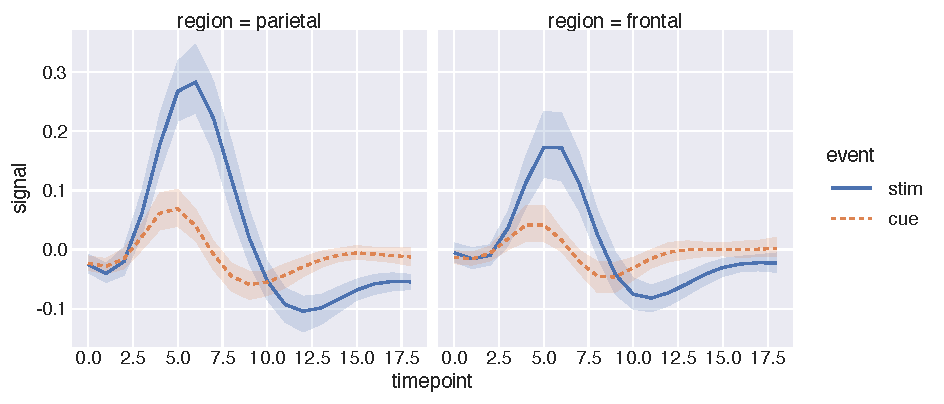
\includegraphics[width=\textwidth]{figures/fig-relplot.pdf}
  \caption{The \texttt{fmri} \texttt{relplot} example from the seaborn documentation,
  reproduced in reaborn with the identical call. The style mapping, bootstrap
  confidence bands, faceting, and theme are reproduced natively in R.}
  \label{fig:relplot}
\end{figure}

\begin{figure}[t]
  \centering
  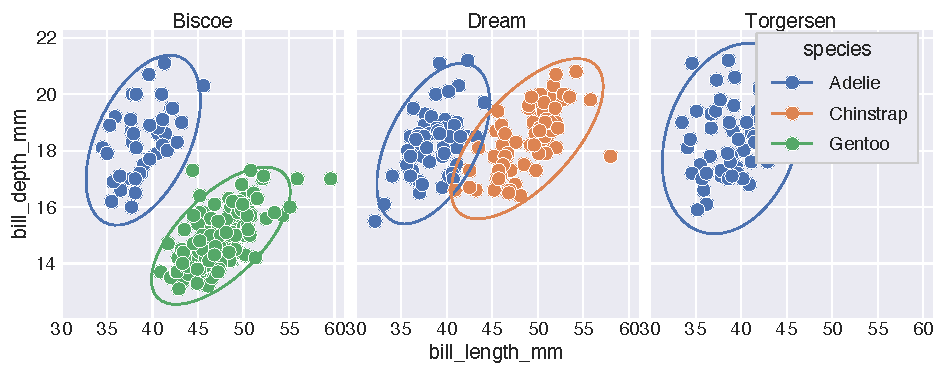
\includegraphics[width=\textwidth]{figures/fig-grammar.pdf}
  \caption{A reaborn one-liner returns a ggplot2 object, so native
  grammar-of-graphics layers compose directly onto it. Here a \texttt{scatterplot()}
  call is extended with ggplot2's \texttt{stat\_ellipse()} and
  \texttt{facet\_wrap(\textasciitilde island)}.}
  \label{fig:grammar}
\end{figure}

\section{State of the field}

Because ggplot2 is a low-level grammar, a rich ecosystem of higher-level helpers has
grown around it to supply opinionated defaults and reduce boilerplate: ggpubr wraps
ggplot2 into publication-ready calls with statistical annotations \citep{ggpubr},
GGally adds pairs and correlation matrices via \texttt{ggpairs} \citep{ggally},
ggdist and the easystats \texttt{see} package add distribution and
model-visualization geoms \citep{kay2024ggdist, ludecke2021see}, cowplot and
patchwork compose multi-panel figures \citep{wilke2024cowplot, patchwork}, and
lattice offers an alternative trellis system \citep{sarkar2008lattice}. Each of
these is built on, and returns, ggplot2 or grid objects, but none reproduces
seaborn's public API---its named functions, argument names, defaults, and specific
statistics. The reverse bridge, calling seaborn from R via reticulate
\citep{reticulate}, requires a Python runtime and yields static matplotlib raster
output rather than grammar-composable ggplot2 objects. The closest conceptual
precedent runs in the opposite direction: plotnine, a port of ggplot2 to Python
\citep{kibirige2025plotnine}. reaborn fills the symmetric and, to our knowledge,
first faithful seaborn-API port to R whose every plot is a ggplot2 object, thereby
unifying the opinionated-defaults and grammar-of-graphics approaches that seaborn's
author described as separate.

\section{Availability, quality, and reproducibility}

reaborn is released under the BSD 3-Clause licence (the same licence as seaborn) and
is developed openly at \url{https://github.com/shawntz/reaborn}, with full
documentation, tutorials, and a function reference at \url{https://reaborn.org}. The
package is feature-complete across seaborn's relational, distributional, categorical,
regression, matrix, and multi-panel families. Quality is maintained through
continuous integration across platforms, a clean \texttt{R CMD check}, and an
extensive automated test suite. A distinguishing element of the test suite is a
\emph{fidelity} component that verifies, against the reference implementations, that
palettes, kernel density estimates, histogram bin edges, and bootstrap intervals
match seaborn---a reproducible benchmark of cross-language equivalence rather than an
aspirational claim. A versioned software archive is available
\href{https://github.com/shawntz/reaborn}{via the repository}.% TODO: replace with Zenodo DOI once minted

\section{AI usage disclosure}

% TODO (author): review and finalize this disclosure to match your actual process before submission.
Generative AI coding assistants were used to assist with portions of the
implementation, test scaffolding, documentation, and the drafting of this manuscript.
All AI-generated output was reviewed, edited, and validated by the author; the core
architectural and design decisions were made by the author, and all
statistical-fidelity claims were verified against the seaborn, SciPy, and NumPy
reference implementations.

\section*{Acknowledgements}

We thank the developers of seaborn, ggplot2, and the broader matplotlib and tidyverse
ecosystems, upon whose work reaborn builds.

\bibliography{references}

\end{document}
